% A simple template for LaTeX documents
% 
% To produce pdf run:
%   $ pdflatex paper.tex 
%

\documentclass[12pt]{article}

% Begin paragraphs with new line
\usepackage{parskip}  

% Change margin size
\usepackage[margin=1in]{geometry}   

% Graphics Example:  (PDF's make for good plots)
\usepackage{graphicx}               
% \centerline{\includegraphics{figure.pdf}}

% Allows hyperlinks
\usepackage{hyperref}

% Blocks of code
\usepackage{listings}
\lstset{basicstyle=\ttfamily, title=\lstname}
% Insert code like this. replace `plot.R` with file name.
% \lstinputlisting{plot.R}

% Supports proof environment
\usepackage{amsthm}

% Allows writing \implies and align*
\usepackage{amsmath}

% Allows mathbb{R}
\usepackage{amsfonts}


%%%%%%%%%%%%%%%%%%%%%%%%%%%%%%%%%%%%%%%%%%%%%%%%%%%%%%%%%%%%

\begin{document}

\begin{center}
    {\Large Assignment 1}\\
    \bigskip
    \hrule
    \medskip
    Clark Fitzgerald\\
    Stats 123
\end{center}

\section*{Makefiles}

Originally designed for compiling large software projects, Makefiles can automate the dependencies between data analysis steps, enabling \textbf{reproducible research}.\footnote{For more on reproducible research, check out the chapter on Open Source Scientific Practice by K. Jarrod Millman and Fernando Perez available at \url{https://osf.io/h9gsd/}.}

\begin{description}
    \item[Statistics-] So hot right now.
    \begin{enumerate}
        \item This is a nested list.
        \item We are shooting for highly nested stuff here.
    \end{enumerate}
    \item[Mathematics-] Always classic.
\end{description}

\vspace{0.3in}

\subsubsection*{R graphics}

Display equations:

\[
    f(x) = x^2 + 5x + \pi
\]

Inline equation $\sum x$, and so on.

You can generate simulated data with R or Python.

\section{R for Graphics}

Here is some R code.

Which generates the corresponding plot:

\centerline{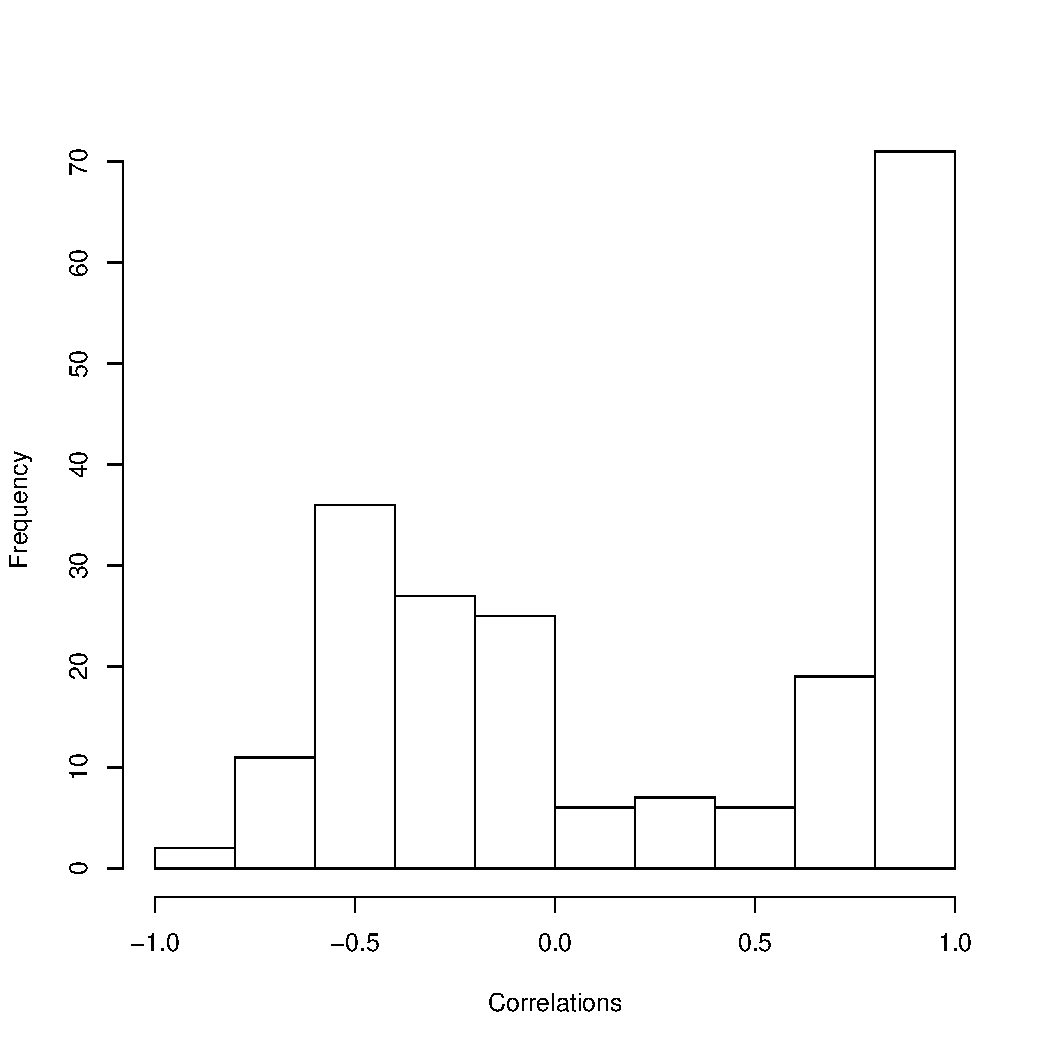
\includegraphics{correlation.pdf}}

\centerline{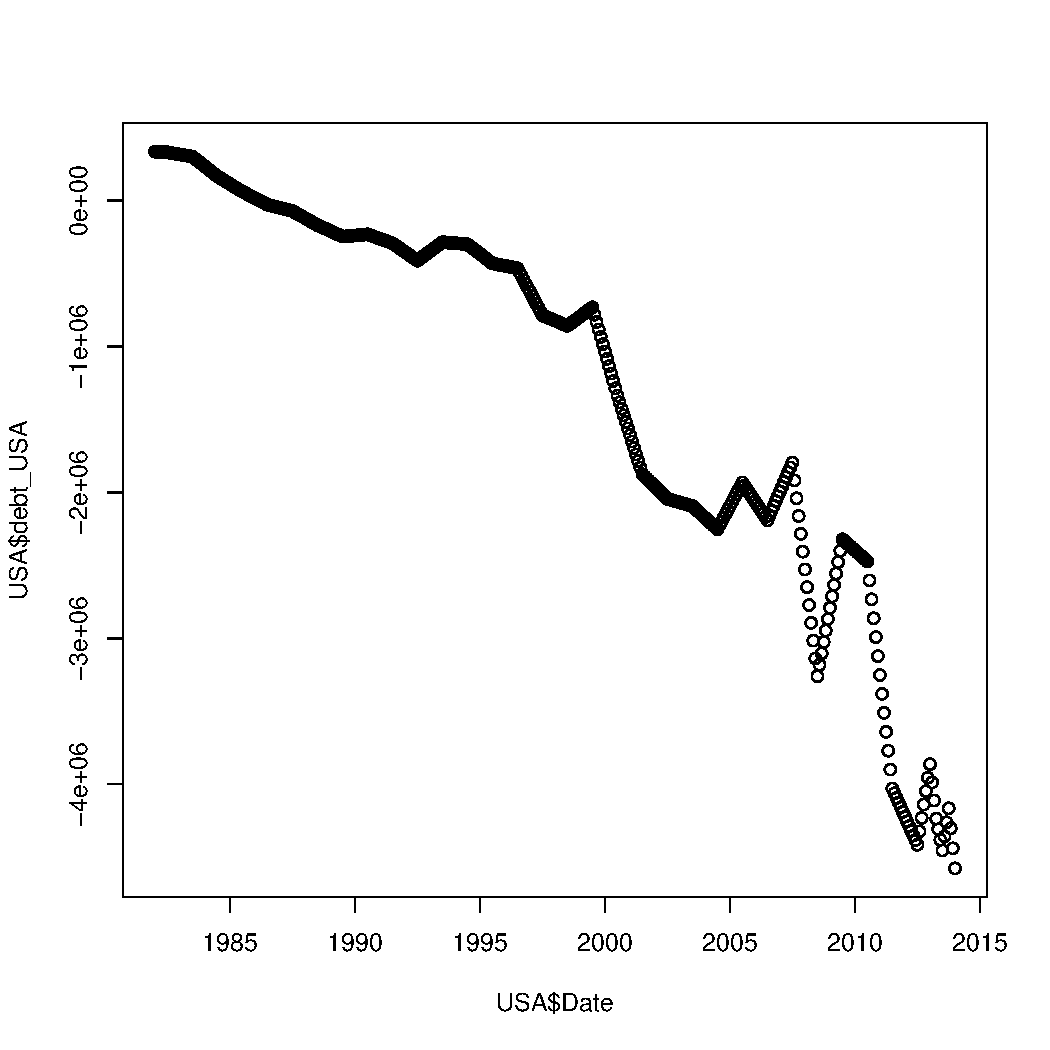
\includegraphics{us_debt.pdf}}

\end{document}
